\documentclass[10pt]{article}

\usepackage[cp1251]{inputenc}
\usepackage[T2A]{fontenc}
\usepackage[russian, english]{babel}

\usepackage{amssymb, amsmath, textcomp, tabularx, graphicx}

\newcolumntype{C}{>{\centering\arraybackslash}X}%

\let \eps \varepsilon

\title{Задание 1}
\author{Коновалов Андрей, 074}
\date{}

\begin{document}

\maketitle

\noindent
\begin{tabularx}{\textwidth}{|C|C|C|C|C|C|C|C|C|}
  \hline
  1 & 2 & 3 & 4 & 5 & 6 & 7 & 8 & $\Sigma$ \\
  \hline
  &&&&&&&& \\
  \hline
\end{tabularx}

\bigskip

{\bf Задача 1}

{\it (i)}
Для того, что бы доказать
$$
  \log{n!} = \Theta (n \log{n})
$$
достаточно показать, что предел
$$
  \lim\limits_{n \to \infty} \frac{\log{n!}}{n \log{n}} =
  \lim\limits_{n \to \infty} \frac{\log{n!}}{\log{n^n}} =
  \lim\limits_{n \to \infty} \frac{a_n}{b_n}
$$
существует, конечен и больше 0, поскольку в этом случае
$$
  \exists C_1 > 0, C_2 > 0: \; C_1 \leq \frac{\log{n!}}{\log{n^n}} \leq C_2
$$
начиная с некоторого $n$.

Поскольку последовательность $b_n$ положительна, неограничена и строго возрастает, то, по теореме Штольца, если существует предел
$$
  \lim\limits_{n \to \infty} \frac{a_n - a_{n - 1}}{b_n - b_{n - 1}}
$$
то существует и предел
$$
  \lim\limits_{n \to \infty} \frac{a_n}{b_n}
$$
причем эти пределы равны.

Вычислим предел
$$\lim\limits_{n \to \infty} \frac{a_n - a_{n - 1}}{b_n - b_{n - 1}} =$$
$$\lim\limits_{n \to \infty} \frac{\log{(n + 1)}}{(n + 1) \log{(n + 1)} - n \log{n}} =$$
$$\lim\limits_{n \to \infty} \frac{\log{(n + 1)}}{\log{(n + 1)} + n \log{\frac{n + 1}{n}}}$$

Заметим, что последовательность
$$
  n \log{\frac{n + 1}{n}} =
  n \log{\left(1 + \frac{1}{n}\right)} =
  n \left(\frac{1}{n} + o\left(\frac{1}{n^2}\right)\right) =
  1 + o\left(\frac{1}{n}\right)
$$
а значит она ограничена.

Получаем, что
$$
  \lim\limits_{n \to \infty} \frac{a_n}{b_n} =
  \lim\limits_{n \to \infty} \frac{a_n - a_{n - 1}}{b_n - b_{n - 1}} =
  1
$$

Значит искомый предел существует, конечен и больше 0.

\medskip

{\bf Задача 2}

{\it (i)}
Запишем рекуррентное соотношение
$$
  T(n) = 5 \cdot T\left(\frac{n}{3}\right) + \Theta(n^2 \log{n})
$$

По определению $\Theta(n^2 \log{n})$
$$
  \exists c_1 > 0, c_2 > 0, n_0 > 0 \;\;\; \forall n \geq n_0 \;\;\; c_1 \leq \frac{\Theta(n^2 \log{n})}{n^2 \log{n}} \leq c_2
$$

Теперь решим следующее рекуррентное соотношение, используя Основную теорему из книги Кормена.
$$
  S(n) = 5 \cdot S\left(\frac{n}{3}\right) + c_1 n^2 \log{n} = a \cdot S\left(\frac{n}{b}\right) + f(n)
$$

Попробуем удовлетворить требованиям третьего случая теоремы.

Заметим, что
$$
  c_1 n^2 \log{n} = f(n) = \Omega(n^{\log_b{a} + \eps}) = \Omega(n^{\log_3{5} + \eps})
$$
при $\eps = 2 - \log_3{5} > 0$.

Проверим выполнение условия
$$
  \exists c < 1, n_0 > 0 \;\;\; \forall n \geq n_0 \;\;\; a f\left(\frac{n}{b}\right) \leq c f(n)
$$

Видно, что это условие выполняется при $c = \frac{5}{9}$:
$$
  5 \left(\frac{n}{3}\right)^2 \log{\frac{n}{3}} \leq \frac{5}{9} n^2 \log{n} \;\;\; \Leftrightarrow \;\;\;
  \log{n} - \log{3} \leq \log{n}
$$

Получаем, что соотношение удовлетворяем условиям теоремы, а значит
$$
  S(n) = \Theta(f(n)) = \Theta(n^2 \log{n})
$$

Поскольку в $S(n)$ была взята константа $c_1$, то
$$
  S(n) \leq T(n)
$$
а значит
$$
  T(n) = \Omega(S(n)) = \Omega(n^2 \log{n})
$$

Аналогично, взяв соотношение с константой $c_2$, получим, что
$$
  T(n) = O(n^2 \log{n})
$$

Итого, получаем, что
$$
  T(n) = \Theta(n^2 \log{n})
$$

\smallskip

{\it (ii)}
Запишем рекуррентное соотношение и решим его, используя Основную теорему из книги Кормена
$$
  T(n) = 4 \cdot T\left(\frac{n}{2}\right) + \Theta(n^2)
$$

Попробуем удовлетворить требованиям второго случая теоремы.

Заметим, что
$$
  \Theta(n^2) = f(n) = \Theta(n^{\log_b{a}}) = \Theta(n^{\log_2{4}}) = \Theta(n^2)
$$

Получаем, что соотношение удовлетворяем условиям теоремы, а значит
$$
  T(n) = \Theta(n^{\log_b{a}} \log{n}) = \Theta(n^2 \log{n})
$$

\smallskip

{\it (iii)}
Запишем рекуррентное соотношение
$$
  T(n) = 9 \cdot T\left(\frac{n}{3}\right) + \Theta(n^2 \sqrt{n} \log^2{n})
$$

Решим его, аналогично пункту {\it (i)} это задачи. Оно удовлетворяет третьему случаю Основной теоремы при
$$
  \eps = \frac{1}{2}, \;\;\; c = \frac{1}{\sqrt{3}}
$$

Соответственно получим решение
$$
  T(n) = \Theta(n^2 \sqrt{n} \log^2{n})
$$

\smallskip

{\it (*)}
Сравнивая асимптотики видим, что лучше выбрать первую или вторую процедуру, чем третью.

\medskip

{\bf Задача 3}

{\it (i)}
Найдем $\Theta$-асимптотику следующего рекуррентного соотношения:
$$
  T(n) = T(\lfloor \sqrt{n} \rfloor) + \Theta(\log^2{n})
$$

Не учитывая округления, сделаем замену переменных $m = \log {n}$, получим
$$
  T(2^m) = T(2^{\frac{m}{2}}) + \Theta(m^2)
$$

Обозначим $S(m) = T(2^{m})$, получим
$$
  S(m) = S\left(\frac{m}{2}\right) + \Theta(m^2)
$$

Используя те же рассуждения, что и в пункте {\it (i)} задачи 2, решим рекуррентное соотношение
$$
  S(m) = S\left(\frac{m}{2}\right) + c m^2
$$

Соотношение удовлетворяет требованиям третьего случая Основной теоремы при
$$
  \eps = 2, \;\;\; c = \frac{1}{4}
$$

Получаем, что
$$
  S(m) = \Theta(m^2)
$$

Возвращаясь к $T(n)$ получаем
$$
  T(n) = T(2^m) = S(m) = \Theta(m^2) = \Theta(\log^2{n})
$$

\medskip

{\bf Задача 4}

{\it (i)}
Назовем следующие операции {\it элементарными битовыми }: сложение двух битов, умножение двух битов, сдвиг любого двоичного числа на 1 бит влево. 

Обозначим $Mult(m)$ как количество элементарных битовых операций, необходимое для перемножения двух $m$-битовых чисел методом Карацубы-Офмана, $Add(m)$ - для сложения, $Shift(m)$ - для сдвига двоичного числа на $m$ бит.

При сложении $m$-битовых двоичных чисел в столбик на каждый бит числа будет приходится не более 2 (учитывая перенос) битовых сложений.
В соответствии с этим $Add(m) = \Theta(m)$.

По определению элементарной битовой операции $Shift(m) = m = \Theta(m)$.

\smallskip

Оценим полное количество элементарных битовых операций при выполнении умножения методом Карацубы-Офмана двух чисел $A$ и $B$ длины $m$.
Будем считать, что $m = 2^k$. Битовую длину числа $x$ будет обозначать как $|x|$.

Представим $A$ и $B$ в виде
$$
  A = a X + b, \;\; B = c X + d
$$
где $X = 2^{\frac{m}{2}}$, $|a| = |b| = |c| = |d| = \frac{m}{2}$.

Шаг умножения методом Карацубы-Офмана запишем следующим образом:
$$(a X + b) (c X + d) = a c X^2 + (a d + b c) X + b d$$
$$a d + b c = (a + b) (c + d) - a c - b d$$

Количество элементарных битовых операций, необходимо для вычисления выражения $\{ expr \}$ будет обозначать как $T(\{ expr \})$.

Получаем, что
\begin{align*}
  T(\{b d\}) = T(\{a c\}) &= Mult\left(\frac{m}{2}\right)\\
  T(\{a c X^2\}) &= T(\{a c\}) + Shift(m)\\
  T(\{a + b\}) = T(\{c + d\}) &= Add\left(\frac{m}{2}\right)\\
  T(\{(a + b) (c + d)\}) &= T(\{a + b\}) + T(\{c + d\}) + Mult\left(\frac{m}{2} + 1\right)\\
  T(\{(a + b) (c + d) - a c - b d\}) &= T(\{(a + b) (c + d)\})\\
  &+ T(\{b d\}) + T(\{a c\}) + 2 \cdot Add\left(m + 2\right)\\
  T(\{(a d + b c) X\} &= T(\{(a + b) (c + d) - a c - b d\}) + Shift\left(\frac{m}{2}\right)
\end{align*}

Учитывая затраты $Add(2m) + Add(2m + 1)$ на сложение трех слагаемых для получения результата, а также оценки для $Add(m)$ и $Shift(m)$ получим
$$
  T(\{(a X + b) (c X + d)\} = Mult(m) = 2 \cdot Mult\left(\frac{m}{2}\right) + Mult\left(\frac{m}{2} + 1\right) + \Theta(m)
$$

В соответствии с рассуждениями на семинаре будем считать, что
$$
  Mult(m) = 3 \cdot Mult\left(\frac{m}{2}\right) + \Theta(m)
$$

\smallskip

{\it (ii)}
Проанализируем полученное рекуррентное соотношение с помощью дерева рекурсии.
Обозначим $Mult(m) = T(m)$.

В соответствии с 4.2 книги Кормена, построим дерево рекурсии для рекуррентного соотношения
$$
  T(m) = 3 \cdot T\left(\frac{m}{2}\right) + c m
$$

\centerline{\includegraphics{{4.2}.png}}

Высота дерева - $\log_2{m}$.
Количество листьев - $3^{log_2{m}} = m^{log_2{3}}$.

Просуммируем времена работы всех уровней дерева:
$$
  T(n) = c m + \left(\frac{3}{2}\right) c m + \left(\frac{3}{2}\right)^2 c m + ... +
    \left(\frac{3}{2}\right)^{log_2{m} - 1} c m + \Theta(m^{log_2{3}}) =
$$
$$
    \sum\limits_{i=0}^{log_2{m} - 1} \left(\frac{3}{2}\right)^i c m + \Theta(m^{log_2{3}}) =
      \frac{\left(\frac{3}{2}\right)^{log_2{m}} - 1}{\frac{3}{2} - 1} c m + \Theta(m^{log_2{3}}) =
$$
$$
  \frac{m^{log_2{\frac{3}{2}}} - 1}{\frac{1}{2}} c m + \Theta(m^{log_2{3}}) =
    2 c m^{log_2{3}} - 2 c m + \Theta(m^{log_2{3}}) =
    O(m^{log_2{3}})
$$

Итого, мы получили оценку сверху $O(m^{log_2{3}})$.

\medskip

{\bf Задача 5}

В соответствии с 4.2 книги Кормена, построим дерево рекурсии для рекуррентного соотношения
$$
  T(n) = 7 \cdot T\left(\frac{n}{2}\right) + c n^2
$$

\centerline{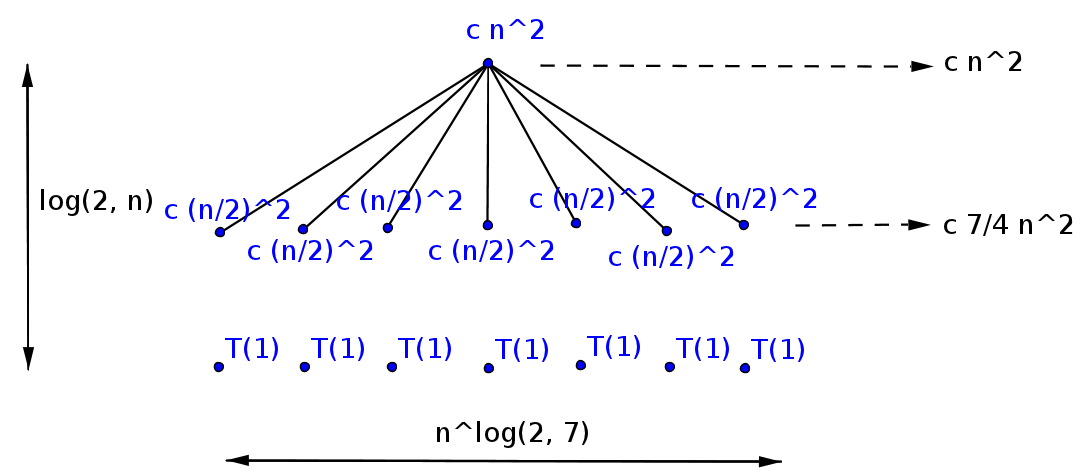
\includegraphics{5.png}}

Просуммируем времена работы всех уровней дерева:
$$
  T(n) = c n^2 + \left(\frac{7}{4}\right) c n^2 + \left(\frac{7}{4}\right)^2 c n^2 + ... +
    \left(\frac{7}{4}\right)^{log_2{n} - 1} c n^2 + \Theta(n^{log_2{7}}) =
$$
$$
    \sum\limits_{i=0}^{log_2{n} - 1} \left(\frac{7}{4}\right)^i c n^2 + \Theta(n^{log_2{7}}) =
      \frac{\left(\frac{7}{4}\right)^{log_2{n}} - 1}{\frac{7}{4} - 1} c n^2 + \Theta(n^{log_2{7}}) =
$$
$$
  \frac{n^{log_2{\frac{7}{4}}} - 1}{\frac{3}{4}} c n^2 + \Theta(n^{log_2{7}}) =
    \frac{4}{3} c n^{log_2{7}} - \frac{4}{3} c n^2 + \Theta(n^{log_2{7}}) =
    O(n^{log_2{7}})
$$

Итого, мы получили оценку сверху $O(n^{log_2{7}})$.

\medskip

{\bf Задача 6}

Покажем, что $a^{15}$ можно вычислить использую лишь 5 умножений.
Справа от выражения записано количество использованных умножений.
\begin{align*}
  a \cdot a \cdot a = a^3 \;\;\; &| \; 2\\
  a^3 \cdot a^3 = a^6 \;\;\; &| \; 1\\
  a^6 \cdot a^6 = a^{12} \;\;\; &| \; 1\\
  a^{12} \cdot a^3 = a^{15} \;\;\; &| \; 1
\end{align*}

\medskip

{\bf Задача 7}

{\it (i)}
Разобьем множество натуральных чисел на интервалы вида
$$\{ [ 2^k, ..., 2^{k + 1} - 1 ] \; | \; k = 0, 1, ... \} = \{ [1], [2, 3], [4, ..., 7], ... \}$$

Докажем, что $l(n) \geq \lambda(n) = \lfloor \log_2{n} \rfloor$ индукцией по номеру интервала $k$.
Заметим, что $\forall n$ из интервала $k$ выполняется $\lambda(n) = k$.

{\it База.}
$$k = 0: l(1) = 1 \geq 0 = \lfloor \log_2{1} \rfloor$$
$$k = 1: l(2) = 2 \geq 1 = \lfloor \log_2{2} \rfloor$$
$$k = 1: l(3) = 3 \geq 1 = \lfloor \log_2{3} \rfloor$$

{\it Переход.}
Пусть $\forall n$ из интервала $k$ выполняется $l(n) \geq \lambda(n) = k$.
Докажем, что $\forall m$ из интервала $k + 1$ выполняется $l(m) \geq \lambda(m)$.

Пусть $m = 2^{k + 1}$.
Расcмотрим произвольную аддитивную цепочку, которая оканчивается числом $m$.
Заметим, что до числа $m$ в цепочке должно было встретиться число из интервала $k$, так как иначе все числа в ней были бы либо больше, чем $m$, и их невозможно было бы использовать при сложении для получения $m$, либо из интервала $t \leq k - 1$, а при их сложении мы не можем получить число из интервала $k + 1$, каковым и является $m$.

По предположению индукции для получения числа из интервала $k$ длина цепочки должна быть $\geq k$.
Что бы получить число $m$ нужно будет совершить еще по крайней мере одно сложение, а значит длина цепочки будет $\geq k + 1 = \lambda(m)$.

Для остальных чисел $m > 2^{k + 1}$ из интервала $k + 1$ последовательно применяем аналогичное рассуждение, только надо учитывать, что для их получения могли использоваться числа из интервала $k + 1$, которые $< m$, но для них ограничение уже доказано, а при их использовании оно не может ухудшиться.

\smallskip

{\it (ii)}
Пусть
$$
  1, a_1, ..., a_r = m, \;\;\; 1, b_1, ..., b_s = n
$$
аддитивные цепочки длины $l(m)$ и $l(n)$ соответственно.

Докажем, что
$$
  l(m n) \leq l(m) + l(n)
$$

Построим цепочку длины $l(m) + l(n)$, заканчивающуюся числом $m n$:
$$
  1, a_1, ..., a_r, a_r b_1, ..., a_r b_s = m n
$$

Строилась она следующим образом. Сначала она повторяла цепочку $a_i$, а затем построение продолжалось аналогично цепочке $b_i$, только вместо числа 1 при суммировании использовалось число $a_r$.

Посколько $l(m n)$ - это цепочка минимальной длины, которая заканчивается числом $m n$, то
$$
  l(m n) \leq l(m) + l(n)
$$

\medskip

{\bf Задача 8}

{\it (i)}
В соответствии с определением из книги Кормена:
$$
  |f| = \sum\limits_{v \in V} f(s, v) = 2 + 2 + 3 = 7
$$

{\it (ii)} Изобразим остаточный граф:

\unitlength=1.3mm
\begin{picture}(190,40)(20,-20)
  \put(18,1){S}
  \put(32,1){D}
  \put(47,1){E}
  \put(66,1){T}
  \put(34,16){A}
  \put(49,16){B}
  \put(64,16){C}
  \put(34,-18){F}
  \put(49,-18){G}
  \put(64,-18){H}
  
  \multiput(35,15)(15,0){3}{\circle*{1}} %A, B, C%
  \multiput(20,0)(15,0){4}{\circle*{1}} %S, D, E, T%
  \multiput(35,-15)(15,0){3}{\circle*{1}} %F, G, H%

  \put(25,8){{\small $3$}} %SA%
  \put(20,0.5){\vector(1,1){14}} %SA%
  \put(28,5.5){{\small $2$}} %AS%
  \put(35,14.5){\vector(-1,-1){14}} %AS%
  
  \put(27,1.5){{\small $3$}} %SD%
  \put(20,0.3){\vector(1,0){14}} %SD%
  \put(27,-2.5){{\small $2$}} %DS%
  \put(35,-0.3){\vector(-1,0){14}} %DS%
  
  \put(28.5,-7){{\small $5$}} %SF%
  \put(20.5,0){\vector(1,-1){14}} %SF%
  \put(25.5,-10){{\small $3$}} %FS%
  \put(35,-15.5){\vector(-1,1){14}} %FS%
  
  \put(42,16.5){{\small $2$}} %AB%
  \put(35,15.3){\vector(1,0){14}} %AB%
  \put(42,12.5){{\small $1$}} %BA%
  \put(50,14.7){\vector(-1,0){14}} %BA%

  \put(36,7){{\small $3$}} %AD%
  \put(35.3,15){\vector(0,-1){14}} %AD%
  \put(32,7){{\small $1$}} %DA%
  \put(34.7,0){\vector(0,1){14}} %DA%
  
  \put(43,5.5){{\small $2$}} %BD%
  \put(50,14.5){\vector(-1,-1){14}} %BD%
  \put(40.5,8.5){{\small $1$}} %DB%
  \put(35,0.5){\vector(1,1){14}} %DB%

  \put(42,1.5){{\small $2$}} %DE%
  \put(35,0.3){\vector(1,0){14}} %DE%
  \put(42,-2.5){{\small $1$}} %ED%
  \put(50,-0.3){\vector(-1,0){14}} %ED%

  \put(32,-8){{\small $4$}} %FD%
  \put(34.7,-15){\vector(0,1){14}} %FD%

  \put(42,-13.5){{\small $2$}} %FG%
  \put(35,-14.7){\vector(1,0){14}} %FG%  
  \put(42,-17.5){{\small $3$}} %GF%
  \put(50,-15.3){\vector(-1,0){14}} %GF%

  \put(57,16.5){{\small $1$}} %BC%
  \put(50,15.3){\vector(1,0){14}} %BC%
  \put(57,12.5){{\small $2$}} %CB%
  \put(65,14.7){\vector(-1,0){14}} %BC%

  \put(51,7){{\small $2$}} %BE%
  \put(50.3,15){\vector(0,-1){14}} %BE%
  \put(47,7){{\small $1$}} %EB%
  \put(49.7,0){\vector(0,1){14}} %EB%
  
  \put(55.5,8.5){{\small $2$}} %EC%
  \put(50,0.5){\vector(1,1){14}} %EC%
  \put(58,5.5){{\small $1$}} %CE%
  \put(65,14.5){\vector(-1,-1){14}} %CE%
  
  \put(57,1.5){{\small $1$}} %ET%
  \put(50,0.3){\vector(1,0){14}} %ET%
  \put(57,-2.5){{\small $2$}} %TE%
  \put(65,-0.3){\vector(-1,0){14}} %TE%
  
  \put(51,-8){{\small $1$}} %EG%
  \put(50.3,0){\vector(0,-1){14}} %EG%
  \put(47,-8){{\small $2$}} %GE%
  \put(49.7,-15){\vector(0,1){14}} %GE%
  
  \put(55.5,-6.5){{\small $1$}} %GT%
  \put(50,-14.5){\vector(1,1){14}} %GT%
  \put(58,-9){{\small $1$}} %TG%
  \put(65,-0.5){\vector(-1,-1){14}} %TG%

  \put(57,-13.5){{\small $4$}} %GH%
  \put(50,-14.7){\vector(1,0){14}} %GH%
  \put(57,-17.5){{\small $1$}} %HG%
  \put(65,-15.3){\vector(-1,0){14}} %HG%

  \put(66,7){{\small $3$}} %CT%
  \put(65.3,15){\vector(0,-1){14}} %CT%
  \put(62,7){{\small $3$}} %TC%
  \put(64.7,0){\vector(0,1){14}} %TC%
  
  \put(66,-8){{\small $1$}} %TH%
  \put(65.3,0){\vector(0,-1){14}} %TH%
  \put(62,-8){{\small $2$}} %HT%
  \put(64.7,-15){\vector(0,1){14}} %HT%
\end{picture}

\smallskip

{\it (iii)}
Нет, так как существует дополняющий путь $SDET$.

\smallskip

{\it (iv)}
С помощью алгоритма Форда-Фалкерсона найдем максимальный поток в заданной сети.
На каждом шаге будет построен остаточный граф и, поиском в глубину, найден дополняющий путь.

В качестве сертификата выполнения поиска в глубину, будут приведены пометки, оставленные после его выполнения.
Пометки будут записаны как индексы букв, обозначающих вершины и имеют следующее соответствие с пометками, описанными в книге Кормена: нет пометки - белая вершина, 1 - серая вершина, 2 - черная вершина.

Так же необходимо сказать, что исходящие из вершины ребра перебираются при поиске в глубину, будучи отсортироваными по часовой стрелке, начиная с полуночи.

Остаточные графы пошагово:

\unitlength=1.3mm
\begin{picture}(190,40)(20,-20)
  \put(18,1){$S_1$}
  \put(34,16){$A_1$}
  \put(49,16){$B_1$}
  \put(64,16){$C_1$}
  \put(32,1){D}
  \put(47,1){E}
  \put(34,-18){F}
  \put(49,-18){G}
  \put(64,-18){H}
  \put(66,1){$T_1$}
  
  \multiput(35,15)(15,0){3}{\circle*{1}} %A, B, C%
  \multiput(20,0)(15,0){4}{\circle*{1}} %S, D, E, T%
  \multiput(35,-15)(15,0){3}{\circle*{1}} %F, G, H%

  \put(25,8){{\small $5$}} %SA%
  \put(20,0.5){\vector(1,1){14}} %SA%
  
  \put(27,1.5){{\small $5$}} %SD%
  \put(20,0.3){\vector(1,0){14}} %SD%
  
  \put(28.5,-7){{\small $8$}} %SF%
  \put(20.5,0){\vector(1,-1){14}} %SF%
  
  \put(42,16.5){{\small $3$}} %AB%
  \put(35,15.3){\vector(1,0){14}} %AB%

  \put(36,7){{\small $4$}} %AD%
  \put(35.3,15){\vector(0,-1){14}} %AD%
  
  \put(40.5,8.5){{\small $3$}} %DB%
  \put(35,0.5){\vector(1,1){14}} %DB%

  \put(42,1.5){{\small $3$}} %DE%
  \put(35,0.3){\vector(1,0){14}} %DE%

  \put(32,-8){{\small $4$}} %FD%
  \put(34.7,-15){\vector(0,1){14}} %FD%

  \put(42,-13.5){{\small $5$}} %FG%
  \put(35,-14.7){\vector(1,0){14}} %FG%

  \put(57,16.5){{\small $3$}} %BC%
  \put(50,15.3){\vector(1,0){14}} %BC%

  \put(51,7){{\small $3$}} %BE%
  \put(50.3,15){\vector(0,-1){14}} %BE%
  
  \put(55.5,8.5){{\small $3$}} %EC%
  \put(50,0.5){\vector(1,1){14}} %EC%
  
  \put(57,1.5){{\small $3$}} %ET%
  \put(50,0.3){\vector(1,0){14}} %ET%
  
  \put(47,-8){{\small $3$}} %GE%
  \put(49.7,-15){\vector(0,1){14}} %GE%
  
  \put(55.5,-6.5){{\small $2$}} %GT%
  \put(50,-14.5){\vector(1,1){14}} %GT%

  \put(57,-13.5){{\small $5$}} %GH%
  \put(50,-14.7){\vector(1,0){14}} %GH%

  \put(66,7){{\small $6$}} %CT%
  \put(65.3,15){\vector(0,-1){14}} %CT%
  
  \put(62,-8){{\small $3$}} %HT%
  \put(64.7,-15){\vector(0,1){14}} %HT%
\end{picture}

Дополняющий путь $SABCT$.

\unitlength=1.3mm
\begin{picture}(190,40)(20,-20)
  \put(18,1){$S_1$}
  \put(34,16){$A_1$}
  \put(49,16){$B_1$}
  \put(64,16){$C_1$}
  \put(32,1){$D_1$}
  \put(47,1){$E_1$}
  \put(34,-18){F}
  \put(49,-18){G}
  \put(64,-18){H}
  \put(66,1){$T_1$}
  
  \multiput(35,15)(15,0){3}{\circle*{1}} %A, B, C%
  \multiput(20,0)(15,0){4}{\circle*{1}} %S, D, E, T%
  \multiput(35,-15)(15,0){3}{\circle*{1}} %F, G, H%

  \put(25,8){{\small $2$}} %SA%
  \put(20,0.5){\vector(1,1){14}} %SA%
  \put(28,5.5){{\small $3$}} %AS%
  \put(35,14.5){\vector(-1,-1){14}} %AS%
  
  \put(27,1.5){{\small $5$}} %SD%
  \put(20,0.3){\vector(1,0){14}} %SD%
  
  \put(28.5,-7){{\small $8$}} %SF%
  \put(20.5,0){\vector(1,-1){14}} %SF%
  
  \put(42,12.5){{\small $3$}} %BA%
  \put(50,14.7){\vector(-1,0){14}} %BA%

  \put(36,7){{\small $4$}} %AD%
  \put(35.3,15){\vector(0,-1){14}} %AD%
  
  \put(40.5,8.5){{\small $3$}} %DB%
  \put(35,0.5){\vector(1,1){14}} %DB%

  \put(42,1.5){{\small $3$}} %DE%
  \put(35,0.3){\vector(1,0){14}} %DE%

  \put(32,-8){{\small $4$}} %FD%
  \put(34.7,-15){\vector(0,1){14}} %FD%

  \put(42,-13.5){{\small $5$}} %FG%
  \put(35,-14.7){\vector(1,0){14}} %FG%

  \put(57,12.5){{\small $3$}} %CB%
  \put(65,14.7){\vector(-1,0){14}} %BC%

  \put(51,7){{\small $3$}} %BE%
  \put(50.3,15){\vector(0,-1){14}} %BE%
  
  \put(55.5,8.5){{\small $3$}} %EC%
  \put(50,0.5){\vector(1,1){14}} %EC%
  
  \put(57,1.5){{\small $3$}} %ET%
  \put(50,0.3){\vector(1,0){14}} %ET%
  
  \put(47,-8){{\small $3$}} %GE%
  \put(49.7,-15){\vector(0,1){14}} %GE%
  
  \put(55.5,-6.5){{\small $2$}} %GT%
  \put(50,-14.5){\vector(1,1){14}} %GT%

  \put(57,-13.5){{\small $5$}} %GH%
  \put(50,-14.7){\vector(1,0){14}} %GH%

  \put(66,7){{\small $3$}} %CT%
  \put(65.3,15){\vector(0,-1){14}} %CT%
  \put(62,7){{\small $3$}} %TC%
  \put(64.7,0){\vector(0,1){14}} %TC%
  
  \put(62,-8){{\small $3$}} %HT%
  \put(64.7,-15){\vector(0,1){14}} %HT%
\end{picture}

Дополняющий путь $SADBECT$.

\unitlength=1.3mm
\begin{picture}(190,40)(20,-20)
  \put(18,1){$S_1$}
  \put(34,16){$A_2$}
  \put(49,16){$B_1$}
  \put(64,16){$C_1$}
  \put(31,1){$D_1$}
  \put(46,1){$E_1$}
  \put(34,-18){F}
  \put(49,-18){G}
  \put(64,-18){H}
  \put(66,1){$T_1$}
  
  \multiput(35,15)(15,0){3}{\circle*{1}} %A, B, C%
  \multiput(20,0)(15,0){4}{\circle*{1}} %S, D, E, T%
  \multiput(35,-15)(15,0){3}{\circle*{1}} %F, G, H%

  \put(28,5.5){{\small $5$}} %AS%
  \put(35,14.5){\vector(-1,-1){14}} %AS%
  
  \put(27,1.5){{\small $5$}} %SD%
  \put(20,0.3){\vector(1,0){14}} %SD%
  
  \put(28.5,-7){{\small $8$}} %SF%
  \put(20.5,0){\vector(1,-1){14}} %SF%
  
  \put(42,12.5){{\small $3$}} %BA%
  \put(50,14.7){\vector(-1,0){14}} %BA%

  \put(36,7){{\small $2$}} %AD%
  \put(35.3,15){\vector(0,-1){14}} %AD%
  \put(32,7){{\small $2$}} %DA%
  \put(34.7,0){\vector(0,1){14}} %DA%
  
  \put(43,5.5){{\small $2$}} %BD%
  \put(50,14.5){\vector(-1,-1){14}} %BD%
  \put(40.5,8.5){{\small $1$}} %DB%
  \put(35,0.5){\vector(1,1){14}} %DB%

  \put(42,1.5){{\small $3$}} %DE%
  \put(35,0.3){\vector(1,0){14}} %DE%

  \put(32,-8){{\small $4$}} %FD%
  \put(34.7,-15){\vector(0,1){14}} %FD%

  \put(42,-13.5){{\small $5$}} %FG%
  \put(35,-14.7){\vector(1,0){14}} %FG%

  \put(57,12.5){{\small $3$}} %CB%
  \put(65,14.7){\vector(-1,0){14}} %BC%

  \put(51,7){{\small $1$}} %BE%
  \put(50.3,15){\vector(0,-1){14}} %BE%
  \put(47,7){{\small $2$}} %EB%
  \put(49.7,0){\vector(0,1){14}} %EB%
  
  \put(55.5,8.5){{\small $1$}} %EC%
  \put(50,0.5){\vector(1,1){14}} %EC%
  \put(58,5.5){{\small $2$}} %CE%
  \put(65,14.5){\vector(-1,-1){14}} %CE%
  
  \put(57,1.5){{\small $3$}} %ET%
  \put(50,0.3){\vector(1,0){14}} %ET%
  
  \put(47,-8){{\small $3$}} %GE%
  \put(49.7,-15){\vector(0,1){14}} %GE%
  
  \put(55.5,-6.5){{\small $2$}} %GT%
  \put(50,-14.5){\vector(1,1){14}} %GT%

  \put(57,-13.5){{\small $5$}} %GH%
  \put(50,-14.7){\vector(1,0){14}} %GH%

  \put(66,7){{\small $1$}} %CT%
  \put(65.3,15){\vector(0,-1){14}} %CT%
  \put(62,7){{\small $5$}} %TC%
  \put(64.7,0){\vector(0,1){14}} %TC%
  
  \put(62,-8){{\small $3$}} %HT%
  \put(64.7,-15){\vector(0,1){14}} %HT%
\end{picture}

Дополняющий путь $SDBECT$.

\unitlength=1.3mm
\begin{picture}(190,40)(20,-20)
  \put(18,1){$S_1$}
  \put(34,16){$A_2$}
  \put(49,16){$B_2$}
  \put(64,16){$C$}
  \put(31,1){$D_1$}
  \put(46,1){$E_1$}
  \put(34,-18){F}
  \put(49,-18){G}
  \put(64,-18){H}
  \put(66,1){$T_1$}
  
  \multiput(35,15)(15,0){3}{\circle*{1}} %A, B, C%
  \multiput(20,0)(15,0){4}{\circle*{1}} %S, D, E, T%
  \multiput(35,-15)(15,0){3}{\circle*{1}} %F, G, H%

  \put(28,5.5){{\small $5$}} %AS%
  \put(35,14.5){\vector(-1,-1){14}} %AS%
  
  \put(27,1.5){{\small $4$}} %SD%
  \put(20,0.3){\vector(1,0){14}} %SD%
  \put(27,-2.5){{\small $1$}} %DS%
  \put(35,-0.3){\vector(-1,0){14}} %DS%
  
  \put(28.5,-7){{\small $8$}} %SF%
  \put(20.5,0){\vector(1,-1){14}} %SF%
  
  \put(42,12.5){{\small $3$}} %BA%
  \put(50,14.7){\vector(-1,0){14}} %BA%

  \put(36,7){{\small $2$}} %AD%
  \put(35.3,15){\vector(0,-1){14}} %AD%
  \put(32,7){{\small $2$}} %DA%
  \put(34.7,0){\vector(0,1){14}} %DA%
  
  \put(43,5.5){{\small $3$}} %BD%
  \put(50,14.5){\vector(-1,-1){14}} %BD%

  \put(42,1.5){{\small $3$}} %DE%
  \put(35,0.3){\vector(1,0){14}} %DE%

  \put(32,-8){{\small $4$}} %FD%
  \put(34.7,-15){\vector(0,1){14}} %FD%

  \put(42,-13.5){{\small $5$}} %FG%
  \put(35,-14.7){\vector(1,0){14}} %FG%

  \put(57,12.5){{\small $3$}} %CB%
  \put(65,14.7){\vector(-1,0){14}} %BC%

  \put(47,7){{\small $3$}} %EB%
  \put(49.7,0){\vector(0,1){14}} %EB%
  
  \put(58,5.5){{\small $3$}} %CE%
  \put(65,14.5){\vector(-1,-1){14}} %CE%
  
  \put(57,1.5){{\small $3$}} %ET%
  \put(50,0.3){\vector(1,0){14}} %ET%
  
  \put(47,-8){{\small $3$}} %GE%
  \put(49.7,-15){\vector(0,1){14}} %GE%
  
  \put(55.5,-6.5){{\small $2$}} %GT%
  \put(50,-14.5){\vector(1,1){14}} %GT%

  \put(57,-13.5){{\small $5$}} %GH%
  \put(50,-14.7){\vector(1,0){14}} %GH%

  \put(62,7){{\small $6$}} %TC%
  \put(64.7,0){\vector(0,1){14}} %TC%
  
  \put(62,-8){{\small $3$}} %HT%
  \put(64.7,-15){\vector(0,1){14}} %HT%
\end{picture}

Дополняющий путь $SDET$.

\unitlength=1.3mm
\begin{picture}(190,40)(20,-20)
  \put(18,1){$S_1$}
  \put(34,16){$A_2$}
  \put(49,16){$B_2$}
  \put(64,16){$C$}
  \put(31,1){$D_2$}
  \put(46,1){$E_2$}
  \put(34,-18){$F_1$}
  \put(49,-18){$G_1$}
  \put(64,-18){H}
  \put(66,1){$T_1$}
  
  \multiput(35,15)(15,0){3}{\circle*{1}} %A, B, C%
  \multiput(20,0)(15,0){4}{\circle*{1}} %S, D, E, T%
  \multiput(35,-15)(15,0){3}{\circle*{1}} %F, G, H%

  \put(28,5.5){{\small $5$}} %AS%
  \put(35,14.5){\vector(-1,-1){14}} %AS%
  
  \put(27,1.5){{\small $1$}} %SD%
  \put(20,0.3){\vector(1,0){14}} %SD%
  \put(27,-2.5){{\small $4$}} %DS%
  \put(35,-0.3){\vector(-1,0){14}} %DS%
  
  \put(28.5,-7){{\small $8$}} %SF%
  \put(20.5,0){\vector(1,-1){14}} %SF%
  
  \put(42,12.5){{\small $3$}} %BA%
  \put(50,14.7){\vector(-1,0){14}} %BA%

  \put(36,7){{\small $2$}} %AD%
  \put(35.3,15){\vector(0,-1){14}} %AD%
  \put(32,7){{\small $2$}} %DA%
  \put(34.7,0){\vector(0,1){14}} %DA%
  
  \put(43,5.5){{\small $3$}} %BD%
  \put(50,14.5){\vector(-1,-1){14}} %BD%

  \put(42,-2.5){{\small $3$}} %ED%
  \put(50,-0.3){\vector(-1,0){14}} %ED%

  \put(32,-8){{\small $4$}} %FD%
  \put(34.7,-15){\vector(0,1){14}} %FD%

  \put(42,-13.5){{\small $5$}} %FG%
  \put(35,-14.7){\vector(1,0){14}} %FG%

  \put(57,12.5){{\small $3$}} %CB%
  \put(65,14.7){\vector(-1,0){14}} %BC%

  \put(47,7){{\small $3$}} %EB%
  \put(49.7,0){\vector(0,1){14}} %EB%
  
  \put(58,5.5){{\small $3$}} %CE%
  \put(65,14.5){\vector(-1,-1){14}} %CE%
  
  \put(57,-2.5){{\small $3$}} %TE%
  \put(65,-0.3){\vector(-1,0){14}} %TE%
  
  \put(47,-8){{\small $3$}} %GE%
  \put(49.7,-15){\vector(0,1){14}} %GE%
  
  \put(55.5,-6.5){{\small $2$}} %GT%
  \put(50,-14.5){\vector(1,1){14}} %GT%

  \put(57,-13.5){{\small $5$}} %GH%
  \put(50,-14.7){\vector(1,0){14}} %GH%

  \put(62,7){{\small $6$}} %TC%
  \put(64.7,0){\vector(0,1){14}} %TC%
  
  \put(62,-8){{\small $3$}} %HT%
  \put(64.7,-15){\vector(0,1){14}} %HT%
\end{picture}

Дополняющий путь $SFGT$.

\unitlength=1.3mm
\begin{picture}(190,40)(20,-20)
  \put(18,1){$S_1$}
  \put(34,16){$A_2$}
  \put(49,16){$B_2$}
  \put(64,16){$C$}
  \put(31,1){$D_2$}
  \put(46,1){$E_2$}
  \put(34,-18){$F_1$}
  \put(49,-18){$G_1$}
  \put(64,-18){$H_1$}
  \put(66,1){$T_1$}
  
  \multiput(35,15)(15,0){3}{\circle*{1}} %A, B, C%
  \multiput(20,0)(15,0){4}{\circle*{1}} %S, D, E, T%
  \multiput(35,-15)(15,0){3}{\circle*{1}} %F, G, H%

  \put(28,5.5){{\small $5$}} %AS%
  \put(35,14.5){\vector(-1,-1){14}} %AS%
  
  \put(27,1.5){{\small $1$}} %SD%
  \put(20,0.3){\vector(1,0){14}} %SD%
  \put(27,-2.5){{\small $4$}} %DS%
  \put(35,-0.3){\vector(-1,0){14}} %DS%
  
  \put(28.5,-7){{\small $6$}} %SF%
  \put(20.5,0){\vector(1,-1){14}} %SF%
  \put(25.5,-10){{\small $2$}} %FS%
  \put(35,-15.5){\vector(-1,1){14}} %FS%
  
  \put(42,12.5){{\small $3$}} %BA%
  \put(50,14.7){\vector(-1,0){14}} %BA%

  \put(36,7){{\small $2$}} %AD%
  \put(35.3,15){\vector(0,-1){14}} %AD%
  \put(32,7){{\small $2$}} %DA%
  \put(34.7,0){\vector(0,1){14}} %DA%
  
  \put(43,5.5){{\small $3$}} %BD%
  \put(50,14.5){\vector(-1,-1){14}} %BD%

  \put(42,-2.5){{\small $3$}} %ED%
  \put(50,-0.3){\vector(-1,0){14}} %ED%

  \put(32,-8){{\small $4$}} %FD%
  \put(34.7,-15){\vector(0,1){14}} %FD%

  \put(42,-13.5){{\small $3$}} %FG%
  \put(35,-14.7){\vector(1,0){14}} %FG%
  \put(42,-17.5){{\small $2$}} %GF%
  \put(50,-15.3){\vector(-1,0){14}} %GF%

  \put(57,12.5){{\small $3$}} %CB%
  \put(65,14.7){\vector(-1,0){14}} %BC%

  \put(47,7){{\small $3$}} %EB%
  \put(49.7,0){\vector(0,1){14}} %EB%
  
  \put(58,5.5){{\small $3$}} %CE%
  \put(65,14.5){\vector(-1,-1){14}} %CE%
  
  \put(57,-2.5){{\small $3$}} %TE%
  \put(65,-0.3){\vector(-1,0){14}} %TE%
  
  \put(47,-8){{\small $3$}} %GE%
  \put(49.7,-15){\vector(0,1){14}} %GE%
  
  \put(58,-9){{\small $2$}} %TG%
  \put(65,-0.5){\vector(-1,-1){14}} %TG%

  \put(57,-13.5){{\small $5$}} %GH%
  \put(50,-14.7){\vector(1,0){14}} %GH%

  \put(62,7){{\small $6$}} %TC%
  \put(64.7,0){\vector(0,1){14}} %TC%
  
  \put(62,-8){{\small $3$}} %HT%
  \put(64.7,-15){\vector(0,1){14}} %HT%
\end{picture}

Дополняющий путь $SFGHT$.

\unitlength=1.3mm
\begin{picture}(190,40)(20,-20)
  \put(18,1){$S_2$}
  \put(34,16){$A_2$}
  \put(49,16){$B$}
  \put(64,16){$C$}
  \put(31,1){$D_2$}
  \put(46,1){$E$}
  \put(34,-18){$F_2$}
  \put(49,-18){$G$}
  \put(64,-18){$H$}
  \put(66,1){$T$}
  
  \multiput(35,15)(15,0){3}{\circle*{1}} %A, B, C%
  \multiput(20,0)(15,0){4}{\circle*{1}} %S, D, E, T%
  \multiput(35,-15)(15,0){3}{\circle*{1}} %F, G, H%

  \put(28,5.5){{\small $5$}} %AS%
  \put(35,14.5){\vector(-1,-1){14}} %AS%
  
  \put(27,1.5){{\small $1$}} %SD%
  \put(20,0.3){\vector(1,0){14}} %SD%
  \put(27,-2.5){{\small $4$}} %DS%
  \put(35,-0.3){\vector(-1,0){14}} %DS%
  
  \put(28.5,-7){{\small $3$}} %SF%
  \put(20.5,0){\vector(1,-1){14}} %SF%
  \put(25.5,-10){{\small $5$}} %FS%
  \put(35,-15.5){\vector(-1,1){14}} %FS%
  
  \put(42,12.5){{\small $3$}} %BA%
  \put(50,14.7){\vector(-1,0){14}} %BA%

  \put(36,7){{\small $2$}} %AD%
  \put(35.3,15){\vector(0,-1){14}} %AD%
  \put(32,7){{\small $2$}} %DA%
  \put(34.7,0){\vector(0,1){14}} %DA%
  
  \put(43,5.5){{\small $3$}} %BD%
  \put(50,14.5){\vector(-1,-1){14}} %BD%

  \put(42,-2.5){{\small $3$}} %ED%
  \put(50,-0.3){\vector(-1,0){14}} %ED%

  \put(32,-8){{\small $4$}} %FD%
  \put(34.7,-15){\vector(0,1){14}} %FD%

  \put(42,-17.5){{\small $5$}} %GF%
  \put(50,-15.3){\vector(-1,0){14}} %GF%

  \put(57,12.5){{\small $3$}} %CB%
  \put(65,14.7){\vector(-1,0){14}} %BC%

  \put(47,7){{\small $3$}} %EB%
  \put(49.7,0){\vector(0,1){14}} %EB%
  
  \put(58,5.5){{\small $3$}} %CE%
  \put(65,14.5){\vector(-1,-1){14}} %CE%
  
  \put(57,-2.5){{\small $3$}} %TE%
  \put(65,-0.3){\vector(-1,0){14}} %TE%
  
  \put(47,-8){{\small $3$}} %GE%
  \put(49.7,-15){\vector(0,1){14}} %GE%
  
  \put(58,-9){{\small $2$}} %TG%
  \put(65,-0.5){\vector(-1,-1){14}} %TG%

  \put(57,-13.5){{\small $2$}} %GH%
  \put(50,-14.7){\vector(1,0){14}} %GH%
  \put(57,-17.5){{\small $3$}} %HG%
  \put(65,-15.3){\vector(-1,0){14}} %HG%

  \put(62,7){{\small $6$}} %TC%
  \put(64.7,0){\vector(0,1){14}} %TC%
  
  \put(66,-8){{\small $3$}} %TH%
  \put(65.3,0){\vector(0,-1){14}} %TH%
\end{picture}

Получаем, что максимальный поток $6 + 3 + 2 + 3 = 14$.

\end{document}
